\pdfoutput=1
\documentclass{article}

\input{preamble/preamble.tex}
\input{preamble/preamble_math}
\input{preamble/definitions_basic}
\input{preamble/minimalist_biblatex}

\addbibresource{bibs/references}

\crefformat{equation}{(#2#1#3)}
\crefformat{figure}{Figure~#2#1#3}
\crefformat{table}{Table~#2#1#3}
\crefname{example}{Example}{Examples}
\crefname{lemma}{Lemma}{Lemmas}
\crefname{cor}{Corollary}{Corollaries}
\crefname{theorem}{Theorem}{Theorems}
\crefname{assumption}{Assumption}{Assumptions}

\usepackage{enumitem}
\usepackage[separate-uncertainty=true,multi-part-units=single]{siunitx}
\usepackage{tikz}
\usetikzlibrary{arrows.meta, positioning, shapes.geometric}

\usepackage[affil-it]{authblk}

\title{Probing Chest X-ray Representations in MedGemma\thanks{Code repository: \url{https://github.com/tnguyen2907/cxr-vlm-interp}.}}
\date{}
\author[1]{Trung Nguyen}
\affil[1]{University of Chicago}

\begin{document}
\maketitle

\begin{abstract}
Medical vision-language models are increasingly used for chest X-ray understanding, but it is not always clear where clinically relevant visual information is most accessible inside these models.
This project studies MedGemma, a medical vision-language model from Google that combines a medically trained MedSigLIP image encoder with a decoder-only Gemma language model.
Because MedSigLIP is designed to provide useful medical image embeddings, it is a natural default representation for embedding-based classification.
However, most of MedGemma's parameters lie in the decoder, raising the question of whether chest X-ray findings become more accessible after image tokens pass through the language model.
Using CheXpert+ studies with five chest X-ray findings, I compare logistic-regression probes on the standalone MedSigLIP embedding, representations from several stages inside MedGemma, and zero-shot generative classification from MedGemma next-token probabilities.
In this experiment, the standalone MedSigLIP baseline achieves the best mean AUROC across the five findings.
The result suggests that, for these labels and this probing setup, MedGemma's decoder does not make the findings more linearly separable than the medically trained image encoder.
\end{abstract}

\section{Introduction}

Chest X-ray interpretation is a central task for medical imaging models.
For many downstream applications, a useful model should be able to classify whether a disease or radiographic finding is present in an image, such as cardiomegaly, edema, or pleural effusion.
A common evaluation strategy is to freeze a medical image encoder, extract an image embedding, and train a simple linear classifier on top of that embedding.
This linear probing setup is attractive because it tests whether clinically relevant information is accessible from the representation without requiring full model fine-tuning.

MedGemma is a medical vision-language model built from Gemma 3, and its visual understanding is powered by MedSigLIP, a medically tuned SigLIP-derived image encoder \citep{medgemma2025}.
MedSigLIP is first adapted for medical image-text representation learning, using a mixture that preserves general SigLIP capability while adding medical image-text data.
MedGemma then reuses this medical vision encoder and continues multimodal training so that Gemma can consume the resulting image tokens.
The MedGemma report presents MedSigLIP as a strong standalone encoder for downstream medical image tasks, including chest X-ray classification.
However, as these image tokens pass through MedGemma's decoder-only language model, their representations are enriched and may differ from the original image embedding.

This motivates the main question of this report:
\emph{is the standalone MedSigLIP embedding the best place to probe for chest X-ray findings, or do intermediate MedGemma decoder representations make these findings more linearly separable?}
This question is motivated by work showing that autoregressive transformers can enrich residual-stream representations during factual recall \citep{geva2023dissecting}.
Although chest X-ray representation learning is different from text-only factual recall, the result suggests a plausible mechanism: a decoder may reorganize information while processing a sequence.
Given the size of MedGemma's decoder relative to the image encoder, my initial hypothesis was that the decoder could reorganize image-token representations using learned language and medical priors, improving linear separability.
However, the empirical result does not support that hypothesis in this setting: the MedSigLIP baseline remains the strongest representation by mean AUROC.
This suggests that adapting visual tokens for next-token prediction does not necessarily make chest X-ray findings more linearly accessible in the decoder residual stream.

\section{MedGemma and MedSigLIP Architecture}

Gemma 3 adds multimodal capability by combining a SigLIP-family vision encoder with a decoder-only language model \citep{gemma32025}.
Images are converted into a sequence of soft image tokens, projected into the language-model hidden space, and then processed by the decoder.
MedGemma adapts this architecture for medical text and imaging tasks \citep{medgemma2025}.
Its associated MedSigLIP encoder is trained as a medical image-text encoder and can also be used independently as a frozen image embedding model.

\begin{figure}[t]
    \centering
    \resizebox{\textwidth}{!}{%
    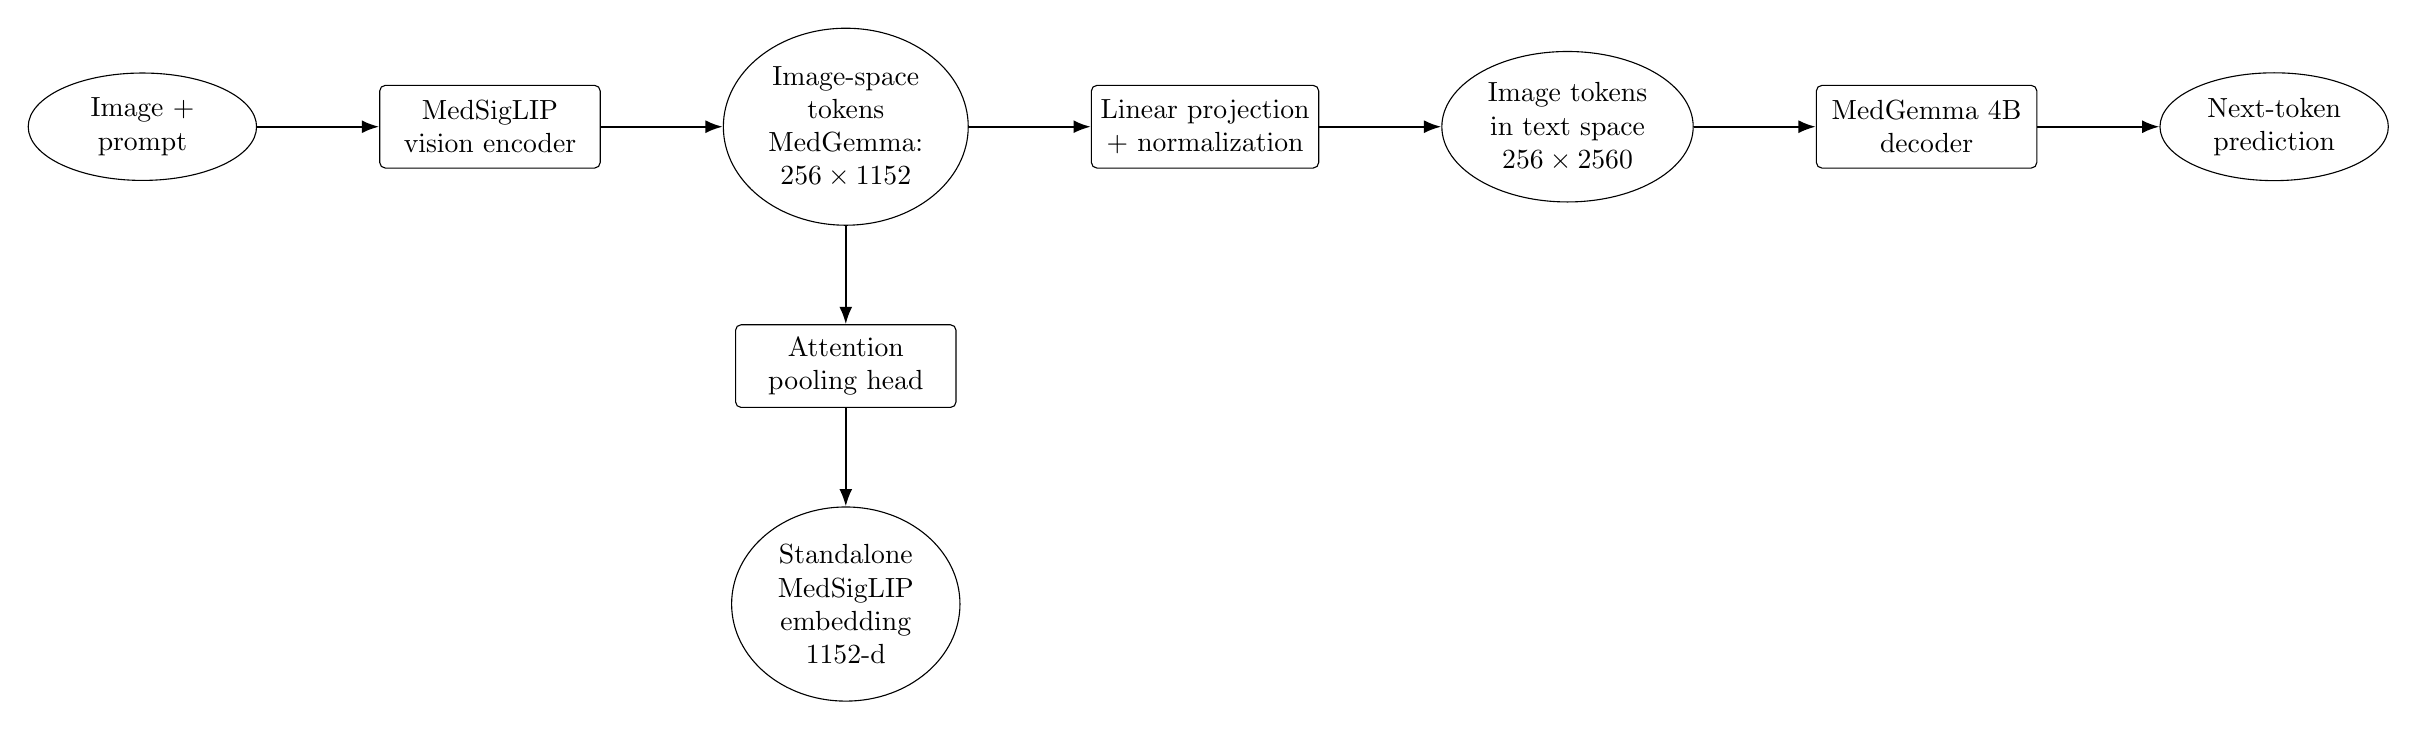
\begin{tikzpicture}[
        node distance=1.25cm and 1.55cm,
        circleNode/.style={ellipse, draw, align=center, minimum width=2.9cm, minimum height=1.05cm},
        blockNode/.style={rectangle, draw, rounded corners=2pt, align=center, minimum width=2.8cm, minimum height=1.05cm},
        arrow/.style={-{Latex[length=2.2mm]}, thick}
    ]
        \node[circleNode] (input) {Image +\\prompt};
        \node[blockNode, right=of input] (encoder) {MedSigLIP\\vision encoder};
        \node[circleNode, right=of encoder] (imageSpace) {Image-space\\tokens\\MedGemma:\\$256 \times 1152$};
        \node[blockNode, right=of imageSpace] (projector) {Linear projection\\+ normalization};
        \node[circleNode, right=of projector] (textSpace) {Image tokens\\in text space\\$256 \times 2560$};
        \node[blockNode, right=of textSpace] (decoder) {MedGemma 4B\\decoder};
        \node[circleNode, right=of decoder] (nextToken) {Next-token\\prediction};
        \node[blockNode, below=1.25cm of imageSpace] (pooling) {Attention\\pooling head};
        \node[circleNode, below=1.25cm of pooling] (standalone) {Standalone\\MedSigLIP\\embedding\\$1152$-d};

        \draw[arrow] (input) -- (encoder);
        \draw[arrow] (encoder) -- (imageSpace);
        \draw[arrow] (imageSpace) -- (projector);
        \draw[arrow] (projector) -- (textSpace);
        \draw[arrow] (textSpace) -- (decoder);
        \draw[arrow] (decoder) -- (nextToken);
        \draw[arrow] (imageSpace) -- (pooling);
        \draw[arrow] (pooling) -- (standalone);
    \end{tikzpicture}}
    \caption{
    Schematic of the MedGemma 4B and standalone MedSigLIP representation paths.
    The MedGemma path projects image tokens into the Gemma hidden space before the decoder.
    The standalone MedSigLIP path applies an attention pooling head to the MedSigLIP vision-token sequence to produce a global image embedding for embedding-based classification.
    }
    \label{fig:architecture}
\end{figure}

The distinction between these two uses of the vision encoder is important for this project.
Both paths begin with the MedSigLIP vision encoder producing a sequence of soft image tokens.
Standalone MedSigLIP pools these image tokens into a single global embedding using a transformer pooling head.
MedGemma instead keeps the image-token sequence, projects it into the Gemma hidden space, and inserts it into the decoder input sequence.
The decoder then processes these visual tokens together with text tokens and ultimately produces next-token probabilities.
This architecture creates several possible probe locations: before the decoder, inside the decoder residual stream, and at the final next-token prediction.

\section{Data}

The experiment uses CheXpert+, a multimodal extension of the CheXpert chest X-ray dataset \citep{chambon2024chexpertplus}.
CheXpert introduced automatically extracted chest X-ray labels with uncertainty annotations and expert comparison for common thoracic findings \citep{irvin2019chexpert}.
Because CheXpert+ was not part of MedGemma model development, it provides a useful external dataset for this probing experiment.
From CheXpert+, 20,000 training studies and 5,000 test studies were sampled, with one image sampled per study.
The evaluation uses five findings that match the chest X-ray findings used in the MedGemma technical report's CheXpert evaluation:
\begin{itemize}[leftmargin=*]
    \item \textbf{Atelectasis}: partial collapse or under-expansion of lung tissue.
    \item \textbf{Cardiomegaly}: an enlarged cardiac silhouette on chest radiograph.
    \item \textbf{Consolidation}: airspace opacity that can occur when alveoli fill with fluid, pus, blood, or cells.
    \item \textbf{Edema}: excess fluid in the lungs, often visible as interstitial or airspace pulmonary edema.
    \item \textbf{Pleural effusion}: fluid collection in the pleural space around the lung.
\end{itemize}
Labels are binarized with a simple rule: definite positive labels are treated as positive, while negative, uncertain, or missing labels are treated as negative.
This label handling makes the task a binary classification problem for each finding, although it does discard the distinction between uncertain and clearly negative labels.

\section{Methods}

\paragraph{Representations.}
Representations are in sequential order from the beginning of the pipeline to the final model output.
This ordering follows the flow shown in \cref{fig:architecture}: first the standalone image embedding, then the projected image tokens before the decoder, then decoder residual states, and finally the model's own zero-shot generative classification score.
The MedGemma representations are extracted from \texttt{google/medgemma-4b-it}.
The reported representations are:
\begin{enumerate}[leftmargin=*]
    \item \textbf{MedSigLIP baseline}: the standalone MedSigLIP image embedding from \texttt{google/medsiglip-448}. This is the main embedding baseline.
    \item \textbf{Pre-decoder image token}: the mean of the projected MedGemma image tokens before they enter the decoder.
    \item \textbf{Mean image token}: the mean over image-token residual states at each decoder layer.
    \item \textbf{Last image token}: the final image-token residual state at each decoder layer.
    \item \textbf{Final prompt token}: the residual state at the final prompt position at each decoder layer.
    \item \textbf{Yes/no logprob}: the zero-shot generative classification score $\log p(\textrm{yes}) - \log p(\textrm{no})$.
\end{enumerate}

\paragraph{Prompts.}
Two prompt orders are used:
\begin{quote}
\small
\texttt{image\_first:}\\
\texttt{\textless image\textgreater}\\
\texttt{Question: Is there [finding] in this image? Answer yes or no.}\\
\texttt{Answer:}

\texttt{text\_first:}\\
\texttt{Question: Is there [finding] in this image? Answer yes or no.}\\
\texttt{\textless image\textgreater}\\
\texttt{Answer:}
\end{quote}
The prompt order matters because MedGemma is decoder-only and therefore causal.
When the image appears before the question, image-token residual states cannot attend to the later text specifying the finding.
When the question appears before the image, image tokens can attend to the finding, so the decoder can in principle form a condition-specific image representation.
This lets us test whether conditioning on the clinical finding makes the image-token or prompt-token representations more linearly separable.
The standalone MedSigLIP baseline and pre-decoder image-token probe do not depend on prompt order in the reported artifacts.

\paragraph{Linear probes.}
For each label and representation, I train a separate logistic-regression probe on the 20,000 training studies and evaluate it on the 5,000 test studies.
The probe is a standard pipeline with feature standardization followed by logistic regression.
The logistic regression uses the LBFGS solver with a maximum of 2,000 iterations.
The evaluation metric is AUROC, matching the MedGemma report's MedSigLIP linear-probe evaluation for chest X-ray classification.

\section{Results}

\Cref{fig:mean-auroc} shows the mean AUROC across the five CheXpert+ findings for each representation stage.
\Cref{tab:mean-results} summarizes the same comparison numerically.

\begin{figure}[t]
    \centering
    \includegraphics[width=\textwidth]{../runs/2026-09-05_imported_artifacts/plots/mean_auroc_over_layers.png}
    \caption{
    Mean AUROC across the five CheXpert+ findings, ordered from earlier to later representation stages.
    Solid curves show layerwise probes, the dashed horizontal line shows the standalone MedSigLIP baseline, and the diamond marker shows direct yes/no log-probability classification.
    }
    \label{fig:mean-auroc}
\end{figure}

\begin{table}[t]
    \centering
    \caption{
    Mean probe performance across the five CheXpert+ findings.
    Bold indicates the best AUROC.
    }
    \label{tab:mean-results}
    \resizebox{\textwidth}{!}{\input{../runs/2026-09-05_imported_artifacts/tables/representation_mean.tex}}
\end{table}

\paragraph{Pre-decoder representations are strongest.}
The standalone MedSigLIP baseline reaches the highest mean AUROC, 0.759.
The pre-decoder image-token probe is close, with mean AUROC 0.755.
This small gap suggests that the projection from MedSigLIP image-token space into the MedGemma text hidden space preserves most of the linearly accessible information needed for these five findings.
In contrast, the best layerwise decoder probes are weaker: the best mean image-token probe reaches mean AUROC 0.731, and the best final prompt-token probe also reaches mean AUROC 0.731.
The per-finding appendix shows the same broad pattern, with the MedSigLIP baseline giving the best AUROC for all five findings.

\paragraph{Decoder processing does not improve linear separability.}
Performance drops considerably as soon as the representation is taken after the first transformer layer of the decoder, compared with the pre-decoder image-token representation.
This suggests that the decoder begins transforming the visual tokens for the objective it was trained for: multimodal next-token prediction and instruction following.
That objective is not necessarily aligned with maintaining a simple linear decision boundary for chest X-ray findings.
In other words, good generative use of visual information does not imply that the same information remains linearly accessible at every residual-stream position.

\paragraph{Layerwise trends differ by representation stage.}
Across layers, the mean image-token and final prompt-token probes generally perform better than the last image-token probes.
The mean image-token and final prompt-token curves fluctuate across layers, but their performance stays roughly level after the initial drop from the pre-decoder representation.
The best mean image-token layer is usually near the beginning of the decoder; pleural effusion is the main exception, where the best mean image-token layers occur near the end.
The best final prompt-token layer varies more across findings.
On the other hand, the last image-token curve has a more distinct trend.
It is strongest in the early layers, where it is closest to the mean image-token and final prompt-token probes, but it becomes weaker deeper into the decoder.

One possible interpretation is that early in the decoder, some finding information is still concentrated in the last image token, while later layers distribute that information across image tokens or route it toward the final prompt token.
However, the mean image-token probe also does not improve with depth, which means simple averaging may not capture the full information distributed across image tokens.
This suggests that more complex pooling methods or token-level probes, such as a transformer pooling head in standalone MedSigLIP, may be needed to test whether clinical information remains present but less accessible through mean pooling.

\paragraph{Zero-shot generative classification is weaker.}
The yes/no log-probability score measures MedGemma's direct prompted classification behavior.
It is weaker than the best embedding-based probes, reaching mean AUROC 0.697 for image-first prompts and 0.667 for text-first prompts.
Cardiomegaly is the main exception where the image-first yes/no score is comparatively close to the pre-decoder representations, but it still does not exceed the MedSigLIP baseline.
This is consistent with the MedGemma report's observation that addressing classification as a zero-shot generative task may underperform embedding-based classification \citep{medgemma2025}.
The text-first prompt is also generally weaker than the image-first prompt in this experiment, with atelectasis as the main exception.
One possible explanation is that, although MedGemma supports interleaved image-text inputs, its training distribution may place images before text more often.
The MedGemma report's image-first chest X-ray classification prompt is consistent with this possibility, but the report does not describe the training prompt format in detail.

\section{Discussion}

The main result is that MedGemma's decoder representations do not outperform representations before the decoder, including the standalone MedSigLIP embedding, for these five CheXpert+ findings.
Zero-shot generative classification also performs worse than training linear classifiers on embeddings from many locations in the model.
Together, these results suggest a gap between optimizing a model for next-token prediction and making clinical findings linearly separable for classification.
The decoder is trained to support multimodal language generation and instruction following, not necessarily to preserve linear disease axes in every residual-stream position.
It may transform visual information into a form that is useful for answering prompts, but less convenient for a simple linear classifier.

Several future directions follow from this result.
First, MedGemma could be fine-tuned directly on the zero-shot generative classification task, and the same probing analysis could then be repeated.
This would test whether supervised adaptation changes the residual-stream representation, reorganizes the image tokens, or improves probe performance.
Second, more mechanistic work could study how clinical information moves across image tokens and prompt tokens inside MedGemma.
Ablation or activation-patching experiments could help identify circuits that carry finding information.
Third, the current probes use simple pooling over image tokens, but richer probes, such as a small transformer over the residual-stream image tokens, could test whether information is distributed across tokens rather than accessible through a mean or last-token summary.
Finally, the experiment should be expanded beyond five findings to larger datasets and the broader CheXpert label set.

\printbibliography

\newpage
\appendix

\section{Per-finding Results}

The following figures and tables show the results for each finding.

\subsection{Atelectasis}

\begin{figure}[!htbp]
    \centering
    \includegraphics[width=\textwidth]{../runs/2026-09-05_imported_artifacts/plots/atelectasis_auroc_over_layers.png}
    \caption{AUROC over representation stage for atelectasis, a finding describing partial lung collapse or under-expansion.}
    \label{fig:atelectasis}
\end{figure}

\begin{table}[!htbp]
    \centering
    \caption{Probe performance for atelectasis. Bold indicates the best AUROC.}
    \resizebox{\textwidth}{!}{\input{../runs/2026-09-05_imported_artifacts/tables/representation_atelectasis.tex}}
\end{table}

\clearpage
\subsection{Cardiomegaly}

\begin{figure}[!htbp]
    \centering
    \includegraphics[width=\textwidth]{../runs/2026-09-05_imported_artifacts/plots/cardiomegaly_auroc_over_layers.png}
    \caption{AUROC over representation stage for cardiomegaly, a finding describing enlargement of the cardiac silhouette.}
    \label{fig:cardiomegaly}
\end{figure}

\begin{table}[!htbp]
    \centering
    \caption{Probe performance for cardiomegaly. Bold indicates the best AUROC.}
    \resizebox{\textwidth}{!}{\input{../runs/2026-09-05_imported_artifacts/tables/representation_cardiomegaly.tex}}
\end{table}

\clearpage
\subsection{Consolidation}

\begin{figure}[!htbp]
    \centering
    \includegraphics[width=\textwidth]{../runs/2026-09-05_imported_artifacts/plots/consolidation_auroc_over_layers.png}
    \caption{AUROC over representation stage for consolidation, an airspace opacity pattern that can reflect alveolar filling.}
    \label{fig:consolidation}
\end{figure}

\begin{table}[!htbp]
    \centering
    \caption{Probe performance for consolidation. Bold indicates the best AUROC.}
    \resizebox{\textwidth}{!}{\input{../runs/2026-09-05_imported_artifacts/tables/representation_consolidation.tex}}
\end{table}

\clearpage
\subsection{Edema}

\begin{figure}[!htbp]
    \centering
    \includegraphics[width=\textwidth]{../runs/2026-09-05_imported_artifacts/plots/edema_auroc_over_layers.png}
    \caption{AUROC over representation stage for edema, a finding describing excess fluid in the lungs.}
    \label{fig:edema}
\end{figure}

\begin{table}[!htbp]
    \centering
    \caption{Probe performance for edema. Bold indicates the best AUROC.}
    \resizebox{\textwidth}{!}{\input{../runs/2026-09-05_imported_artifacts/tables/representation_edema.tex}}
\end{table}

\clearpage
\subsection{Pleural Effusion}

\begin{figure}[!htbp]
    \centering
    \includegraphics[width=\textwidth]{../runs/2026-09-05_imported_artifacts/plots/pleural_effusion_auroc_over_layers.png}
    \caption{AUROC over representation stage for pleural effusion, a finding describing fluid in the pleural space around the lung.}
    \label{fig:pleural-effusion}
\end{figure}

\begin{table}[!htbp]
    \centering
    \caption{Probe performance for pleural effusion. Bold indicates the best AUROC.}
    \resizebox{\textwidth}{!}{\input{../runs/2026-09-05_imported_artifacts/tables/representation_pleural_effusion.tex}}
\end{table}

\end{document}
